\documentclass[12pt,fleqn,answers]{exam}
\usepackage{amssymb}
\usepackage[intlimits]{amsmath}
\usepackage{epsfig}
\usepackage{upgreek}
\usepackage[super]{nth}
\usepackage[colorlinks=true,linkcolor=black,anchorcolor=black,citecolor=black,filecolor=black,menucolor=black,runcolor=black,urlcolor=black]{hyperref}
\usepackage[letterpaper, margin=0.75in]{geometry}
\addpoints
\boxedpoints
\pointsinmargin
\pointname{pts}
\usepackage{tikz}
\usepackage{tkz-euclide}
\usetikzlibrary{shapes.geometric}
\usetikzlibrary{calc}
\usepackage[final]{microtype}
\frenchspacing
\usepackage[american]{babel}
\usepackage[T1]{fontenc}
\usepackage[upright]{fourier}
\usepackage{isomath}
\usepackage{upgreek,amsmath}
\usepackage{graphicx}

\newcommand{\dotprod}{\, {\scriptzcriptztyle\stackrel{\bullet}{{}}}\,}

\newcommand{\reals}{\mathbf{R}}
\newcommand{\lub}{\mathrm{lub}} 
\newcommand{\glb}{\mathrm{glb}} 
\newcommand{\complex}{\mathbf{C}}
\newcommand{\dom}{\mbox{dom}}
\newcommand{\range}{\mbox{range}}
\newcommand{\cover}{{\mathcal C}}
\newcommand{\integers}{\mathbf{Z}}
\newcommand{\vi}{\, \mathbf{i}}
\newcommand{\vj}{\, \mathbf{j}}
\newcommand{\vk}{\, \mathbf{k}}
\newcommand{\bi}{\, \mathbf{i}}
\newcommand{\bj}{\, \mathbf{j}}
\newcommand{\bk}{\, \mathbf{k}}
\DeclareMathOperator{\Arg}{\mathrm{Arg}}
\DeclareMathOperator{\Ln}{\mathrm{Ln}}
\newcommand{\imag}{\, \mathrm{i}}
\newcommand{\erf}{\mathrm{erf}}

\usepackage{graphicx}
\usepackage{color}
%\shadedsolutions
%\definecolor{SolutionColor}{rgb}{1,0.72,0.46} %{0.8,0.9,1}
\newcommand\AM{\textsc{am}}
\newcommand\PM{\textsc{pm}}
     
\newcommand{\quiz}{19}
\newcommand{\term}{Fall}
\newcommand{\due}{Thursday 2 November 13:20}
\newcommand{\class}{MATH 202, Fall \the\year}
\begin{document}
%\large
\vspace{0.1in}
\noindent\makebox[3.0truein][l]{\textbf{\class}}
\textbf{Name:} \hrulefill \\
\noindent \makebox[3.0truein][l]{\textbf{In class work  \quiz}}
\textbf{Row and Seat}:\hrulefill\\

\large
\noindent \emph{“
“Life is full of surprises, but never when you need one.” } \hfill {\sc Calvin (Bill Watterson)}

\vspace{0.1in}

\noindent  In class work  \textbf{\quiz}  has questions \textbf{1} 
through  \textbf{\numquestions} \/ with a total of 
\textbf{\numpoints\/} points. Turn in your work at the end of class 
\emph{on paper}. This assignment is due \emph{\due}.


 

\begin{questions} 

\question [1] Use the fact that for all real $x$ the equation $\displaystyle \mathrm{e}^x = \sum_{k=0}^\infty \frac{1}{k!}  x^k$ is an identity 
 to find a power series representation for $\mathrm{e}^{-x^2} $.
\begin{solution}[2.5in]
Replacing $x$ by $-x^2$ in $\displaystyle \mathrm{e}^x = \sum_{k=0}^\infty \frac{1}{k!}  x^k$ gives the power series
\begin{equation*}
\mathrm{e}^{-x^2} = \sum_{k=0}^\infty \frac{1}{k!}  (-x^2)^k.
\end{equation*}
And this is a power series that only has even powers of the variable $x$. It's optional to do so, but the power series 
can also be expressed as
\begin{equation*}
\mathrm{e}^{-x^2} = \sum_{k=0}^\infty \frac{(-1)^k}{k!}  x^{2 k}.
\end{equation*}
Expressed this way, it's fairly clear that for real $x$, we have an alternating series.

\textbf{Tidbit:} Had I asked for the power series for $\exp(\sin(x))$, we'd have trouble with that. It's certainly 
true that for all real $x$ that
\begin{equation*}
  \mathrm{e}^{\sin(x)} = \sum_{k=0}^\infty \frac{(-1)^k}{k!}  \sin(x)^{2 k}.
\end{equation*}
But this isn't a power series (it's not a sum of nonnegative powers of $x$.) Yes, it's a series in powers of 
$\sin(x)$, but not a series of powers of $x$.
\end{solution}


\question [1] Define a function $\erf$ by the definite integral $\erf(x) = \frac{2}{\sqrt{\uppi}} \large \int_0^x \mathrm{e}^{-t^2} \, \mathrm{d} t$.
Find a power series representation for $\erf$.  Find the radius of convergence of this power series.
\begin{solution}%[3.5in]
We have
\begin{align*}
\erf(x) &= \frac{2}{\sqrt{\uppi}} \large \int_0^x \mathrm{e}^{-t^2} \, \mathrm{d} t, \\
            &= \frac{2}{\sqrt{\uppi}} \large \int_0^x \sum_{k=0}^\infty \frac{(-1)^k}{k!}  t^{2 k} \, \mathrm{d} t, \\
            &= \frac{2}{\sqrt{\uppi}}  \sum_{k=0}^\infty \large \int_0^x \frac{(-1)^k}{k!}  t^{2 k} \, \mathrm{d} t, \\
            &= \frac{2}{\sqrt{\uppi}}  \sum_{k=0}^\infty\frac{(-1)^k}{k!} \large \int_0^x   t^{2 k} \, \mathrm{d} t, \\
            &= \frac{2}{\sqrt{\uppi}}  \sum_{k=0}^\infty\frac{(-1)^k}{k!} \frac{x^{2 k+1}}{2 k + 1}.
\end{align*}
We could use the ratio test, but the theory of power series tells us that the termwise integration does not change
the radius of convergence. So the radius of convergence is infinity.
\end{solution}

\newpage

\question [1]  With a bit of faith and luck, maybe a good approximation to $\erf$ is the sum of its first 101 terms.
Use Desmos to graph this approximation for $-6 < x < 6$.   Actually, the function $\erf$ is known to Desmos. Plot
a graph of both the sum of the first 101 terms of the power series for $\erf$ along with the function $\erf$.
As best you can, reproduce the graphs here.  Incidentally, the sum of the first 101 terms is $\displaystyle \sum_{k=0}^{100}$,
not $\displaystyle \sum_{k=0}^{101}$.


\begin{solution}[1.5in]
For $-5 < x < 5$, the two graphs are so close, I can't tell any difference. Outside this interval, the graphs are wildly different.
The graph of the sum of the first 101 terms of the power series (the red graph) starts to increase super fast past about 6
, but the graph of $\erf$ looks like it has a horizontal asymptote toward infinity.

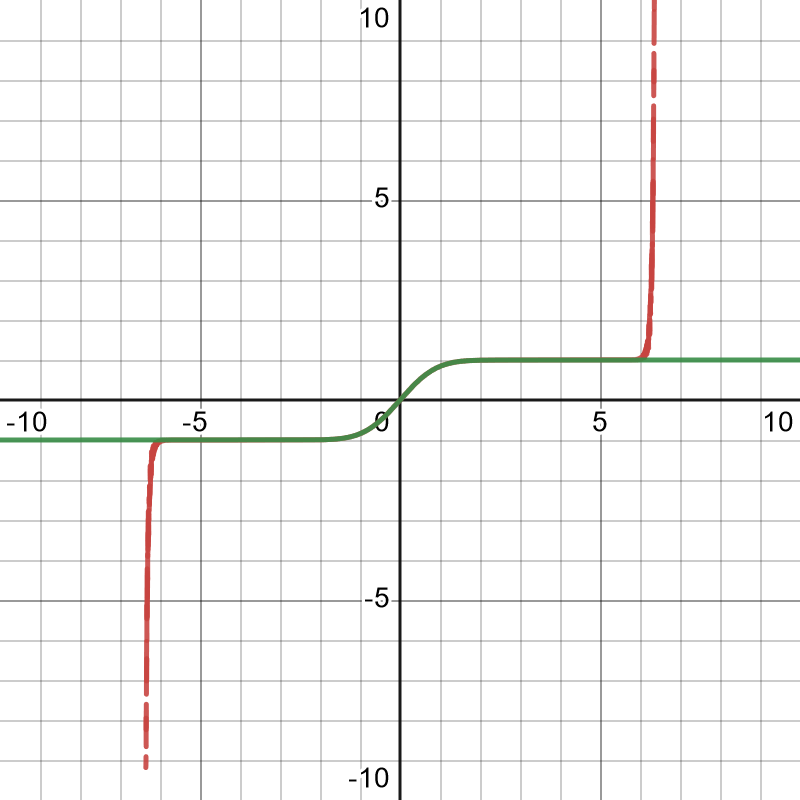
\includegraphics[scale=0.2]{desmos-graph(67).png}

\end{solution}


\question [1] Based on the Desmos graph of $\erf$, what is your conjecture for the value of $\displaystyle \lim_{x \to \infty} \erf(x)$? 


\begin{solution}%[4.5in]
Looking at the graph of $\erf$, I guess that $\displaystyle \lim_{x \to \infty} \erf(x) = 1$.

\end{solution}

\newpage

\question [1]   For ``large'' values of $x$, explain why 
$\frac{2}{\sqrt{\uppi}}  \sum_{k=0}^{N} \frac{(-1)^k}{ (2 k + 1) (k !)}   x^{2 k +1}$ is not a good approximation to $\erf$
no matter how large we make $N$.  

\textbf{Remember:} No matter the degree of a polynomial, its limit toward infinity is determined 
by the term of the polynomial with the highest power.  For example, provided $a_{101} \neq 0$, we have 
\begin{equation*}
  \lim_{x \to \infty}  \left( a_o + a_1 x + a_2 x^2 + \cdots + a_{101} x^{101} \right)  =  
  \lim_{x \to \infty} a_{101} x^{101}  = \begin{cases}  -\infty & a_{101} < 0 \\ \infty & a_{101} > 0 \end{cases}.
\end{equation*}

\begin{solution}[3.5in]
For any integer $N$, we have $$\lim_{x \to \infty} \frac{2}{\sqrt{\uppi}}  \sum_{k=0}^{N} \frac{(-1)^k}{ (2 k + 1) (k !)}   x^{2 k +1} = \begin{cases} \infty & N \text{ is even} \\ -\infty & N \text{ is odd} \end{cases}. $$ But $\displaystyle \lim_{x \to \infty} \erf(x) = 1$. 
So for large $x$,  the graphs of $y = \frac{2}{\sqrt{\uppi}}  \sum_{k=0}^{N} \frac{(-1)^k}{ (2 k + 1) (k !)}   x^{2 k +1}$
and $y  = \erf(x) $ are far far apart, no matter how large we make $N$.  So for sufficiently large $x$ and no matter how 
large we make $N$, the value of $\sum_{k=0}^{N} \frac{(-1)^k}{ (2 k + 1) (k !)}   x^{2 k +1}$ will differ greatly
from $\erf(x)$

\quad Another way to think of this: The only polynomial that has a horizontal asymptote toward infinity is a constant polynomial. So attempting
to approximate a nonconstant function that has a horizontal asymptote toward infinity with a polynomial 
will be wildly inaccurate toward infinity.

\end{solution}

\question  [1] Find a formula for the derivative of $\erf$; that is find a formula for $\erf^\prime$.  Make your formula as ``simple'' as you can.  You might like to return the initial definition as a definite integral; that is $\erf(x) = \frac{2}{\sqrt{\uppi}} \large \int_0^x \mathrm{e}^{-t^2} \, \mathrm{d} t$

\begin{solution} The FTC gives $\erf^\prime(x)  = \frac{2}{\sqrt{\uppi}} \exp(-x^2).$

\end{solution}

\end{questions}
\end{document}
